% Partial trace only. Gaps and crossed strokes do not certify the knot topology.
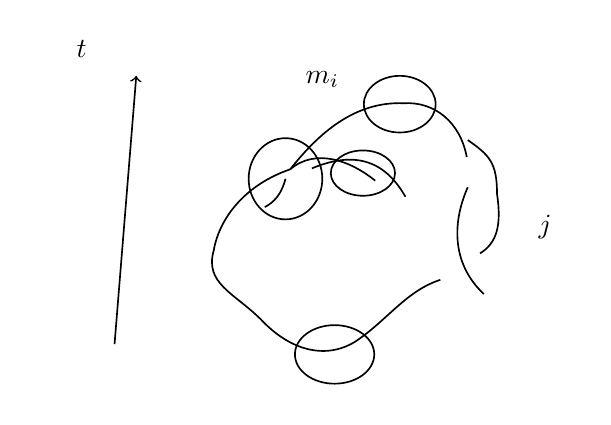
\begin{tikzpicture}[x=0.012cm,y=-0.012cm,line width=0.6pt]
\path[use as bounding box] (0,0) rectangle (588,391);
\draw[->] (92,335)--(115,51);\node at (57,23) {$t$};
\draw (278,150)..controls(231,166)and(203,201)..(197,236)
 ..controls(187,271)and(219,281)..(247,309)
 ..controls(277,341)and(314,352)..(346,333)
 ..controls(380,311)and(400,279)..(437,267);
\draw (278,150)..controls(308,112)and(346,78)..(398,80)
 ..controls(431,78)and(458,100)..(465,137);
\draw (466,119)..controls(489,135)and(497,143)..(497,176)
 ..controls(502,209)and(497,228)..(479,239);
\draw (466,169)..controls(448,210)and(451,252)..(483,282);
\draw (278,150)..controls(305,127)and(342,141)..(368,162);
\draw (301,149)..controls(337,134)and(374,133)..(400,179);
\draw (273,160)..controls(269,176)and(261,185)..(251,190);
\draw (394,81) ellipse[x radius=38,y radius=30];
\draw (273,160) ellipse[x radius=39,y radius=43];
\draw (355,154) ellipse[x radius=34,y radius=24];
\draw (325,346) ellipse[x radius=42,y radius=31];
\node at (312,55) {$m_i$};\node at (548,211) {$j$};
\end{tikzpicture}
